\begin{figure}[H]
\centering
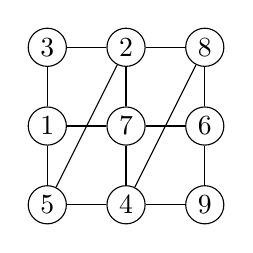
\begin{tikzpicture}
\tikzstyle{vertex}=[draw, circle, inner sep=2pt]
    \node[vertex] (1) at (0,1) {$1$};
    \node[vertex] (2) at (1,2) {$2$};
    \node[vertex] (3) at (0,2) {$3$};
    \node[vertex] (4) at (1,0) {$4$};
    \node[vertex] (5) at (0,0) {$5$};
    \node[vertex] (6) at (2,1) {$6$};
    \node[vertex] (7) at (1,1) {$7$};
    \node[vertex] (8) at (2,2) {$8$};
    \node[vertex] (9) at (2,0) {$9$};

    \draw (6) -- (9);
    \draw (6) -- (8);
    \draw (6) -- (7);
    
    \draw (4) -- (9);
    \draw (4) -- (8);
    \draw (4) -- (7);
    \draw (4) -- (5);
    
    \draw (2) -- (8);
    \draw (2) -- (7);
    \draw (2) -- (5);
    \draw (2) -- (3);
    
    \draw (1) -- (7);
    \draw (1) -- (5);
    \draw (1) -- (3);

\end{tikzpicture}
\label{fig:3n-subgrid}
\caption{Tileable $\Grid_{3 \times n}$ subgraph of $\CGrid$ with one additional edge every column.}
\end{figure}